Here we report an example script where a general illustration of the \textit{easyReporting} is described.

As already mentioned, the class allows to report not only the \gls{cc}, but allows also to add personal titles and personal comments, enhancing the knowledge transfer between the ''back-side'' (the analyst/developer) and the ''front-side'' (the reader) users.
Note that ''back-side'' and ''front-side'' can also be the data analyst and the collaborators, respectively.

\begin{lstlisting}
## Creating report file with default options on global document
rd <- easyreporting$new(filenamepath="./project_report", title="example_report", author=c("Dario Righelli"))

rd$mkdTitle("First Level Title")

rd$mkdGeneralMsg("Here I'm writing a simple paragraph useful to describe my code chunk")

## Leaving the default options to the code chunk
rd$mkdCodeChunkSt()

## Adding a variable assignement
variable <- 1
rd$mkdVariableAssignment("variable", "variable", show=TRUE)
rd$mkdCodeChunkEnd()

## Or i can create my own options for the chunk
rd$mkdTitle("Second Level Title", level=2)
optList <- maketOptionsList(includeFlag=TRUE)
rd$mkdCodeChunkSt(optionsList=optList)
rd$mkdCodeChunkEnd()

## Moreover I can add a list of files to source in che code chunk
rd$mkdCodeChunkSt(optionsList=optList, source.files.list=c("R/cachingFunctions.R", "R/cachingFunctions.R"))
rd$mkdCodeChunkEnd()


rd$mkdCodeChunkComplete(message="a <- 1\nb <- 2\nc <- a+b\n print(c)")


## Otherwise I can make a direct call with all the code chunk and the comment in one call
optList <- makeOptionsList(includeFlag=TRUE, cacheFlag=TRUE)

rd$mkdCodeChunkCommented(commentMsg="This is the comment of the following code chunk",
                    message="a <- 1\nb <- 2\n(c <- a+b)",
                    optionsList=optList,
                    source.files.list=NULL)

## finally I can directly compile my report
rd$compile()
\end{lstlisting}
 
The previous R script leads to automatically produce the following \textit{rmarkddown} file, where it is possible to see at rows 13 and 23 two titles at different levels.
And additionally, starting from row 15 a describing paragraph, representing the additional comments that can added to provide additional explanations to the following \gls{cc}.

\begin{lstlisting}

---
    title: "example_report"
    author: "Dario Righelli"
    date: "`r Sys.Date()`"
    output: rmarkdown::html_document
---

```{r global_options, include=FALSE}
knitr::opts_chunk$set(eval=TRUE, echo=TRUE, warning=FALSE, message=FALSE, include=TRUE, cache=TRUE)
```

# First Level Title

Here I'm writing a simple paragraph useful to describe my code chunk

```{r eval=TRUE, echo=TRUE, warning=FALSE, message=FALSE, include=TRUE, cache=TRUE}

variable <- `variable`
print(variable)

```
## Second Level Title
```{r eval=TRUE, echo=TRUE, warning=FALSE, message=FALSE, include=TRUE, cache=TRUE}

```

```{r eval=TRUE, echo=TRUE, warning=FALSE, message=FALSE, include=TRUE, cache=TRUE}
source("/Users/inzirio/Desktop/gDrive/works/coding/easyreporting/R/cachingFunctions.R")
source("/Users/inzirio/Desktop/gDrive/works/coding/easyreporting/R/cachingFunctions.R")
```

```{r eval=TRUE, echo=TRUE, warning=FALSE, message=FALSE, include=TRUE, cache=TRUE}
a <- 1
b <- 2
c <- a+b
 print(c)
```

This is the comment of the following code chunk

```{r eval=TRUE, echo=TRUE, warning=FALSE, message=FALSE, include=TRUE, cache=TRUE}
a <- 1
b <- 2
(c <- a+b)
```
\end{lstlisting}

Thanks to the \lstinline!rd$compile()! command inside the first script, it automatically produces the final \textit{HTML} \textit{report} illustrated in figure \ref{fig:rrreport}.

Finally, the report in \gls{html} format provides a human readable document, where all the \gls{cc} are highlithed in grey, and the results in white.
Titles and comments are in plain text, highlighting the natural language format of a self-explaining document.

\begin{figure}[H]
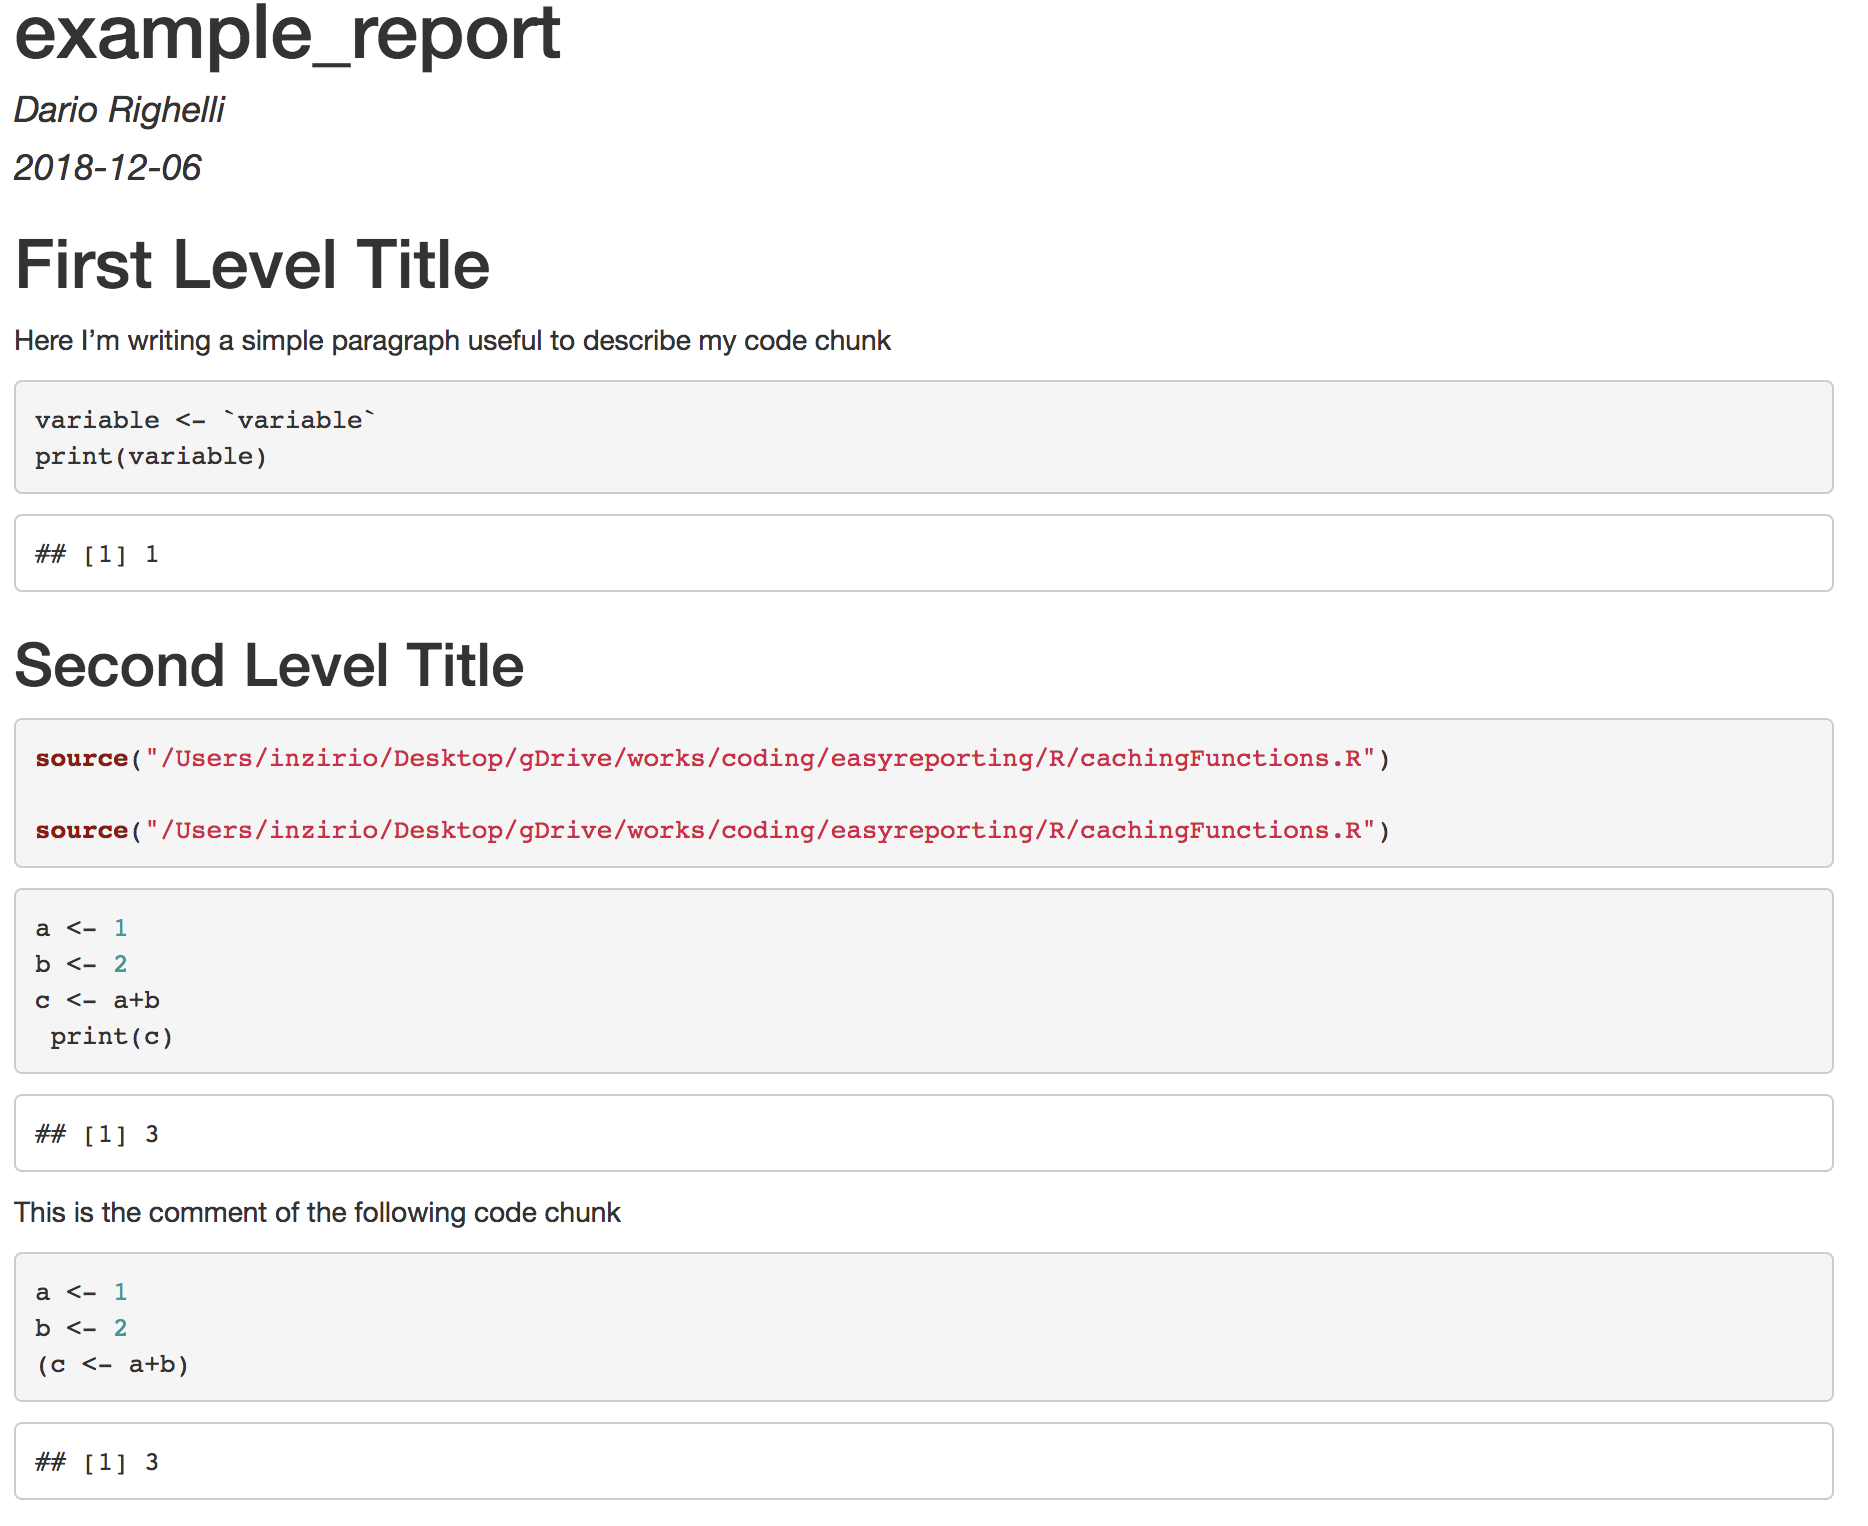
\includegraphics[width=\textwidth, keepaspectratio]{img/rr/report.png}
\caption[html report]{An example HTML report with \textit{easyReporting} R package.}
\label{fig:rrreport}
\centering
\end{figure}